\chapter{引言}
\label{chap:introduction}

\section{游戏背景与规则}
国际象棋影响深远受众广泛,在经历了漫长的传播与演变后形成了今日的规则。
哈罗德·穆雷所著的\textit{A History of Chess} 详细记载了其演变过程与各种游戏规则的变种与分支~\cite{murray2015history}。
在中世纪之后的很长一段时间内,皇后棋子(或者被称为~Amazon~,也即本文中的超级皇后)可以像现代皇后或骑士一样移动,如图~\ref{fig:superQueen},白色圆点代表白色方超级皇后可落子位置。只不过由于其太过强力难以制衡,相对平衡的现代皇后在国际象棋规则中作为正统胜出。
指导老师与笔者受其启发,构思出一款国际象棋衍生游戏—超级皇后对战。
% \begin{figure}[htb]
%   \centering
%   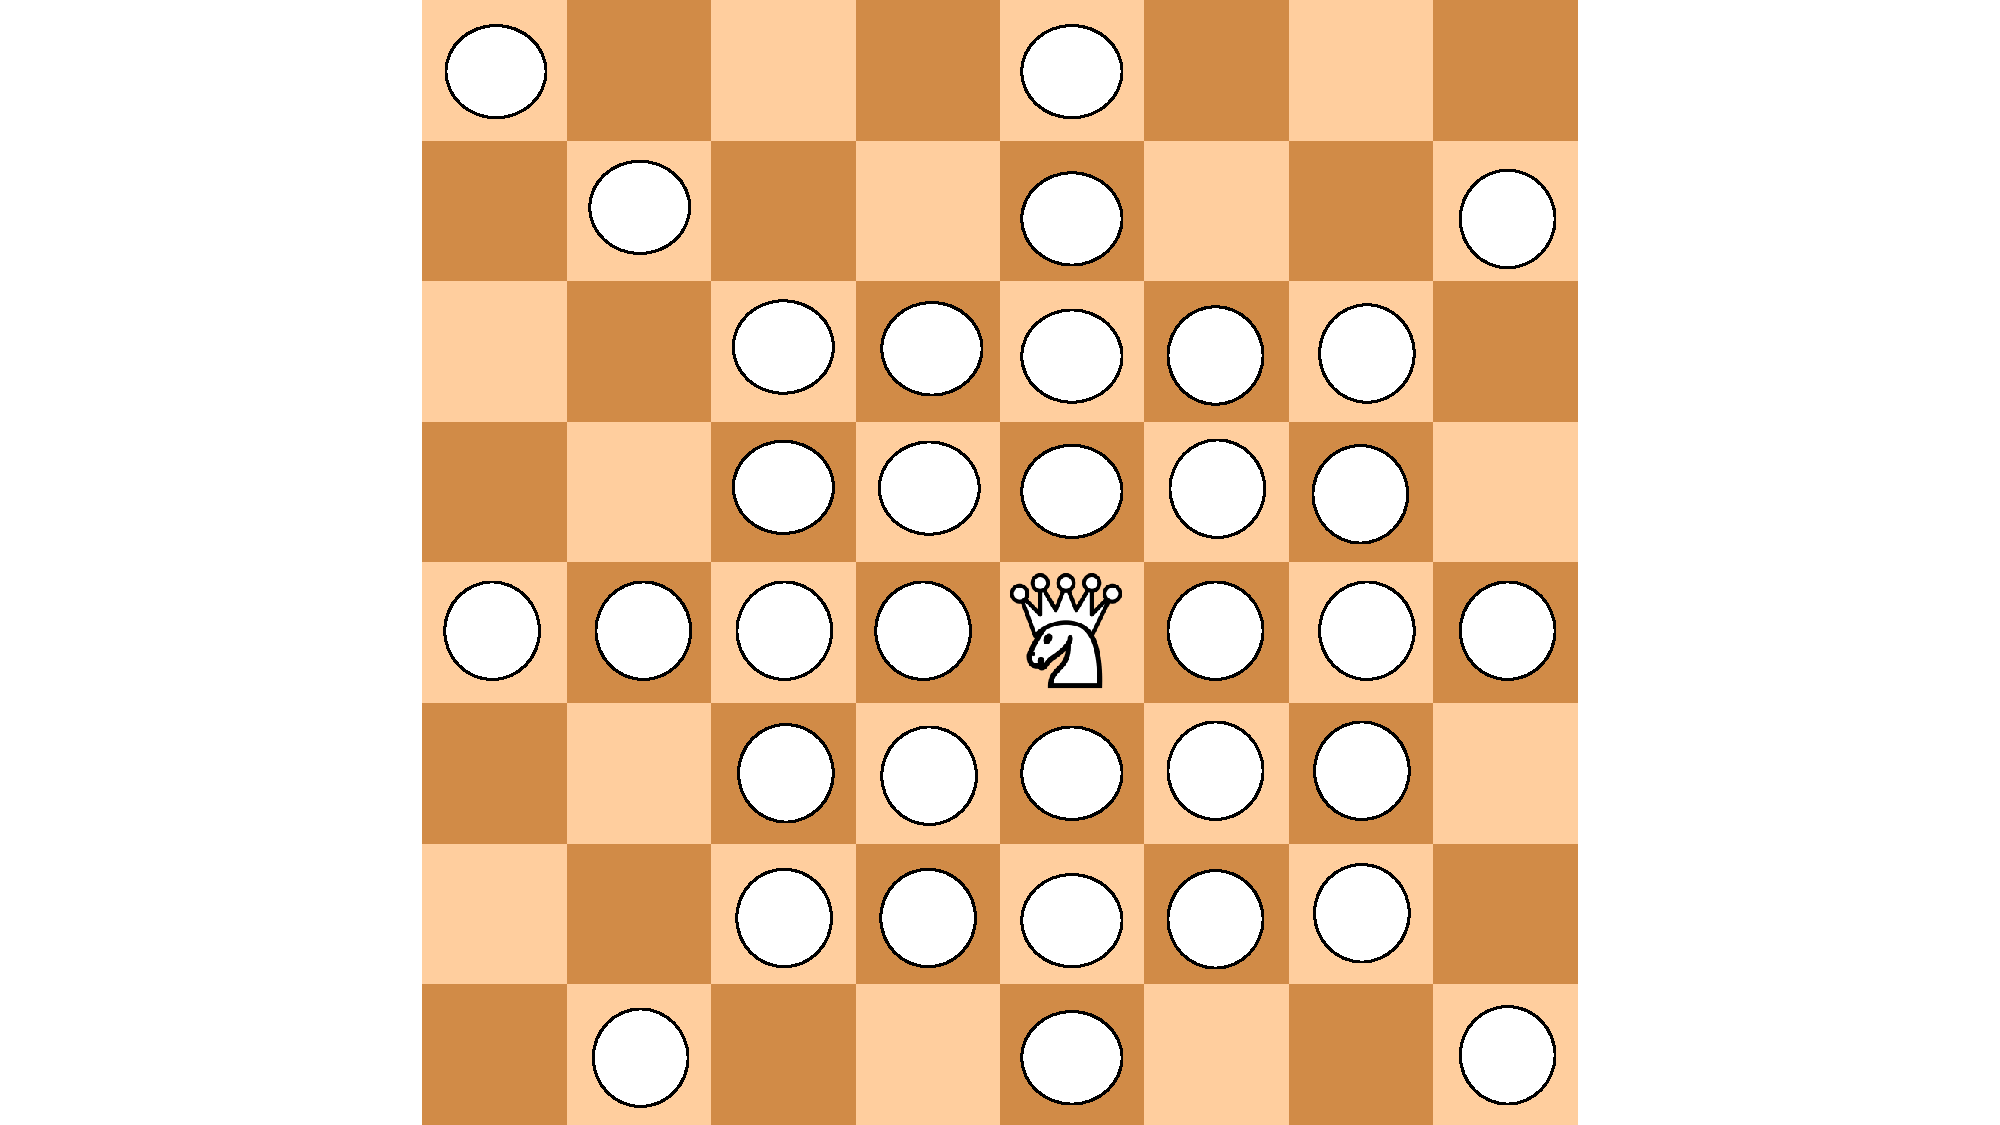
\includegraphics[width=0.7\textwidth]{amazon.pdf}
%   \caption[superQueen]{%
%     超级皇后走法,其可以像皇后与骑士一样移动~\cite{wikiAmazon}。}
%   \label{fig:superQueen}
% \end{figure}
规则描述如下:指定大小的棋盘($8\times8$,$12\times12$等)有黑白两个超级皇后;超级皇后的落子规则可指定,包括皇后走法、骑士走法与混合走法(即超级皇后走法),不可越过移动路线上的对方棋子,不可攻击对方;
每当超级皇后离开当前位置,该位置变为不可落子的死地,但是双方棋子皆可越过死地。
黑白双方超级皇后用如图~\ref{fig:superQueenRules}~所示的黑白图标表示,用黑叉($\mathbf{\times}$)表示死地。胜利条件为封死对方超级皇后的行动。相比于围棋和国际象棋,此游戏的棋面局势与所涉及到的状态空间并不复杂。

% \begin{figure}[htb]
%     \centering
%     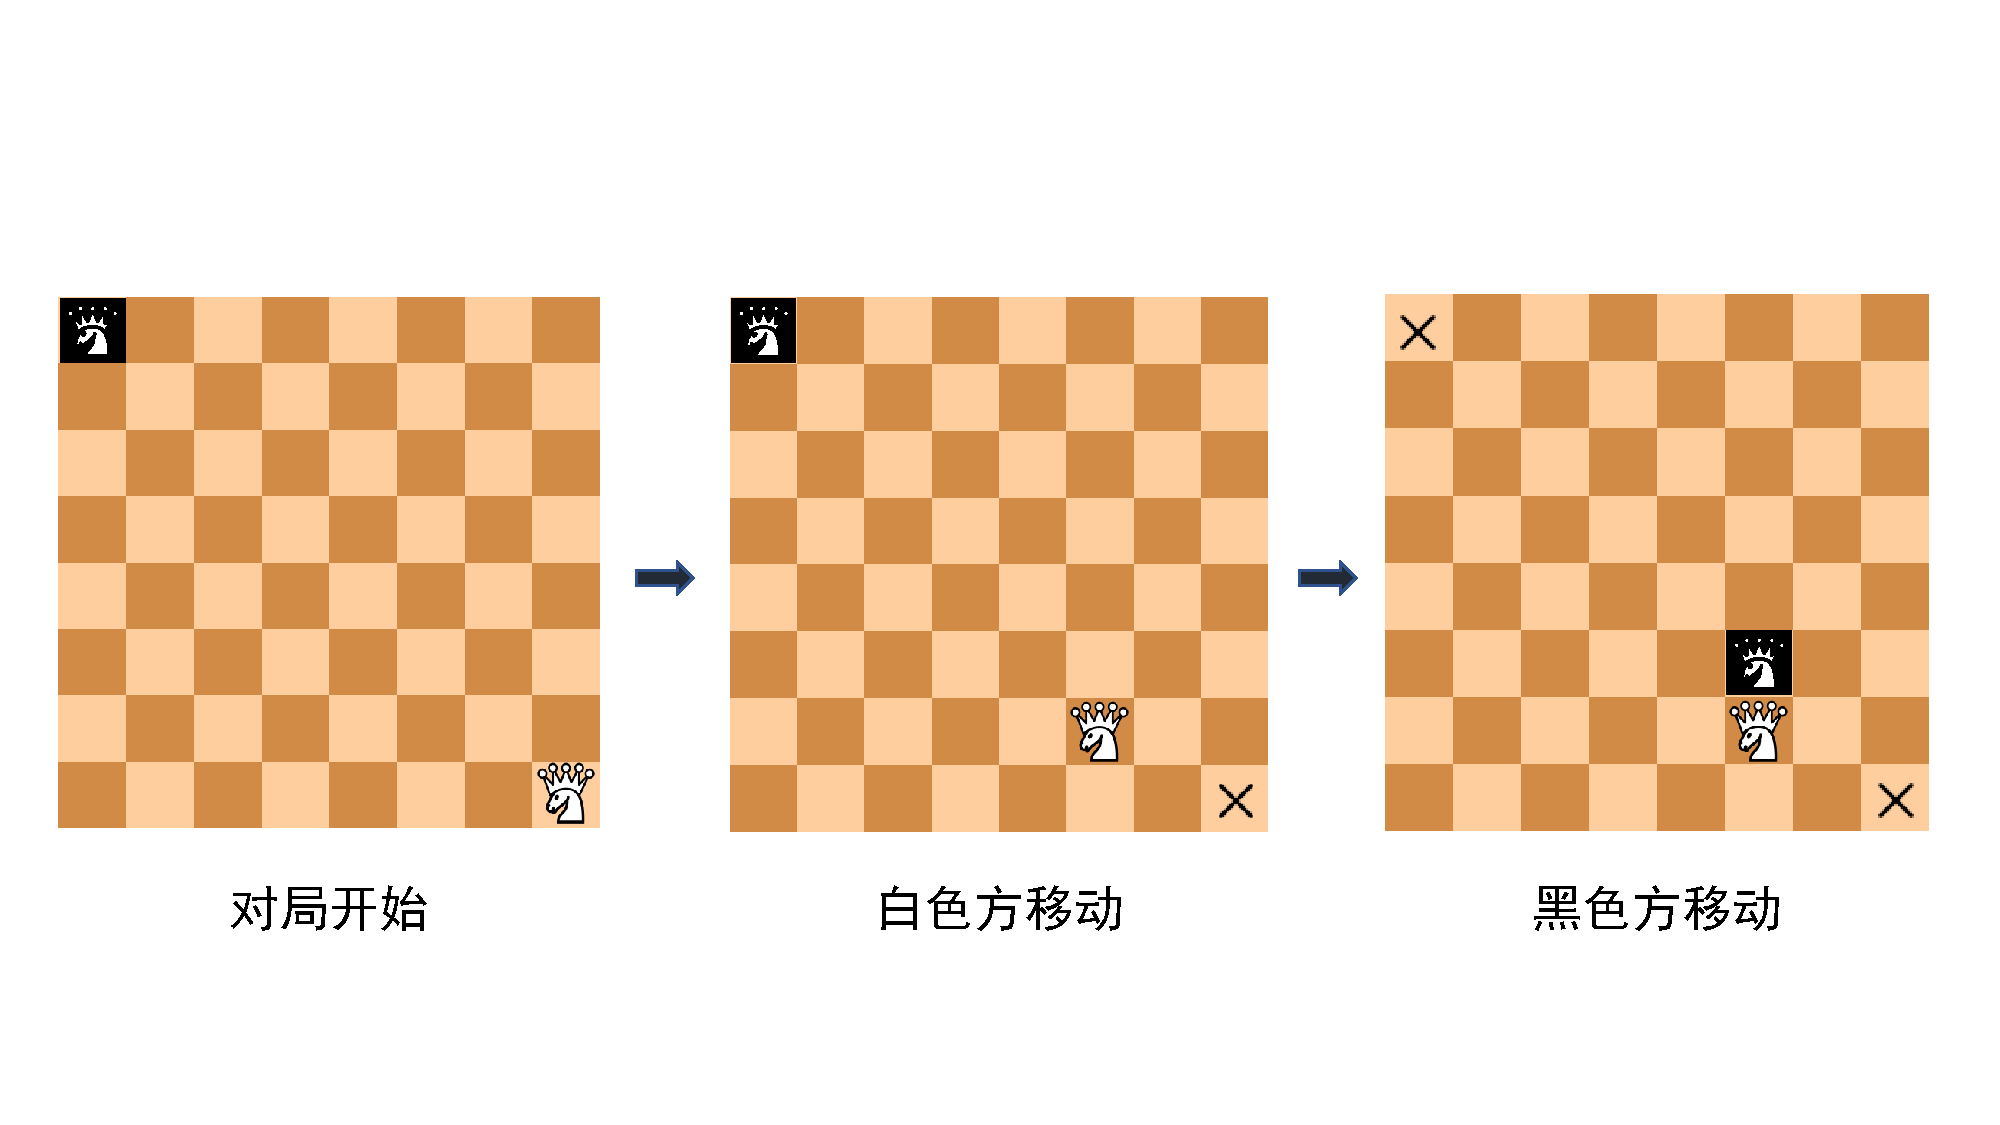
\includegraphics[width=\textwidth]{rules.pdf}
%     \caption[superQueenRules]{%
%       超级皇后对战游戏规则%
%       }
%     \label{fig:superQueenRules}
%   \end{figure}


\section{本文工作}
我们构思出了一款国际象棋衍生游戏,并实现了对战框架,可进行人机对战与电脑AI对战。针对电脑AI玩家,我们设计了以下几种AI:(1)随机玩家(Random Player),顾名思义,其每步动作都基于当前可行走法进行随机选择,此玩家也将作为~baseline~测试其余AI是否有效;
(2)贪婪玩家(Greedy Player),依据评分函数,在每一步选择中都采取在当前状态下最好或最优(即最有利)的走法;(3)alpha-beta~剪枝玩家,采取带~alpha-beta~剪枝的极大极小化算法,对博弈树进行部分搜索得到最佳落子~\cite{russell2010artificial};(4)AlphaZero框架玩家,依据谷歌公司提出来的理论,即结合蒙特卡洛树搜索与深度神经网络进行强化学习的AI训练方法~\cite{Silver1140}。
同时,针对~AlphaZero~框架,由于超级皇后对战与围棋、五子棋、国际象棋在棋面局势评估上具有显著不同,我们还针对其网络结构与初始化设置不同的有效性进行了探索研究。

\section{论文结构}
本文总共包含五章。在第一章中,我们介绍所构思的新游戏背景与规则。此外并介绍了本文的主要工作,最后介绍本文结构。

在第二章中,会介绍本文所设计的新游戏AI涉及到的理论,包括极小化极大算法,alpha-beta~剪枝以及组成~AlphaZero~结构的蒙特卡洛树搜索,深度神经网络与强化学习等基本理论。

在第三章中,会介绍我们的对战框架设计,AI玩家设计与训练方法。

在第四章中,会介绍我们的训练结果与对战实验。

在第五章中,我们会对整个工作进行总结。

